\documentclass[titlepage,a4paper]{article}


\usepackage[spanish,activeacute]{babel}
%\usepackage[margin = 1in]{geometry}
\usepackage{a4wide}
\usepackage{bookmark}
\usepackage{fancyhdr}
\usepackage{graphicx}

\pagestyle{fancy} % Encabezado y pie de página
\fancyhf{}
\fancyhead[L]{TP1  - Grupo: 38}
\fancyhead[R]{Teoría de organización de datos - FIUBA}
\renewcommand{\headrulewidth}{0.4pt}
\fancyfoot[C]{\thepage}
\renewcommand{\footrulewidth}{0.4pt}





\begin{document}

	\begin{titlepage}
		\hfill
\includegraphics[width=6cm]{logofiuba.jpg}
		\center
		\vfill
		\vfill
		\begin{center}
			\begin{Huge}\textbf{Trabajo Práctico Nº 1}\end{Huge}\\
			\vfill
			\begin{huge}Análisis Exploratorio\end{huge}\\
			\vfill
			\begin{Large} Teoría de Organización de Datos\end{Large}\\

			\textbf{Nombre grupo:} "The data inception" \\
			\textbf{Nº grupo: 38}\\
				Todo el trabajo realizado puede encontrarse en el siguiente repositorio de github:\textit{ https://github.com/sebalogue/tp1-datos.git. }
	
			\vfill
			\begin{tabular}{|c|c|c|}
				\hline
				participantes & nº padrón & mail \\ \hline
				LOIS,Lucas Edgardo &[COMPLETAR] &  [COMPLETAR] \\ \hline		
				LOGUERCIO, Sebastian Ismael &[COMPLETAR] &  [COMPLETAR] \\ \hline
				MARIANI, Santiago Tomás &100516 &  santiagomariani2@gmail.com \\ \hline
				MARIJUAN, Magalí & 100070 & maguimar001@gmail.com\\ \hline
				
			\end{tabular}
			\vfill
			\vfill
			\vfill
			\vfill
			\vfill
			\vfill
		\end{center}
	
	\end{titlepage}

	\tableofcontents
	\newpage
	
	\section{Introducción}
	Este trabajo práctico consite en realizar un análisis sobre un conjunto de eventos de web analytics de usuarios que visitaron www.trocafone.com, su plataforma de ecommerce de Brasil.
	
	Para realizar dicho trabajo utilizaremos el lenguaje de programación \textit{Python}. Para el análisis de datos usaremos la librería \textit{Pandas} y para la realización de gráficos utilizaremos las librerías \textit{Matplotlib }y \textit{Seaborn}. Por otro lado, trabajaremos usando el sistema de control de versiones \textit{GIT}	
	
	En nuestra primera experiencia decimos usar la siguiente abstracción para realizar el trabajo práctico: \textbf{preguntar al dataset}, es decir, que en nuestro modelo siempre hacemos preguntas que luego intentaremos responder con los datos que obtendremos del dataset. 
	
	\section{Análisis Preliminar}
	En un primer análisis intentaremos entender cómo esta compuesto el data set. Es decir, cuáles son los eventos que los componenen, cómo interactúan como un conjunto y cuáles son las características propias de cada evento. 
	\subsection{Eventos}
	El dataset contiene los siguiente eventos: 
	\begin{itemize}
	\item Viewed product: El usuario visita una página de producto.
	\item Brand listing: El usuario visita un listado específico de una marca viendo un conjunto de productos.
	\item Visited site: El usuario ingresa al sitio a una determinada url.
	\item Ad campaign hit:  El usuario ingresa al sitio mediante una campana de marketing online.
	\item Generic listing:  El usuario visita la homepage.
	\item Serched products:  El usuario realiza una búsqueda de productos en la interfaz de búsqueda del site.
	\item Search engine hit: El usuario ingresa al sitio mediante un motor de búsqueda web.
	\item Checkout: El usuario ingresa al checkout de compra de un producto.
	\item Staticpage: El usuario visita una página.
	\item Conversion: El usuario realiza una conversión, comprando un producto.
	\item Lead: El usuario se registra para recibir una notificación de disponibilidad de stock, para un producto que no se encontraba disponible en ese momento.
	\newpage
	La cantidad total de eventos es: 	1011288. Los cuales están distribuidos de la siguiente manera. 
	\end{itemize}
	\begin{center}
	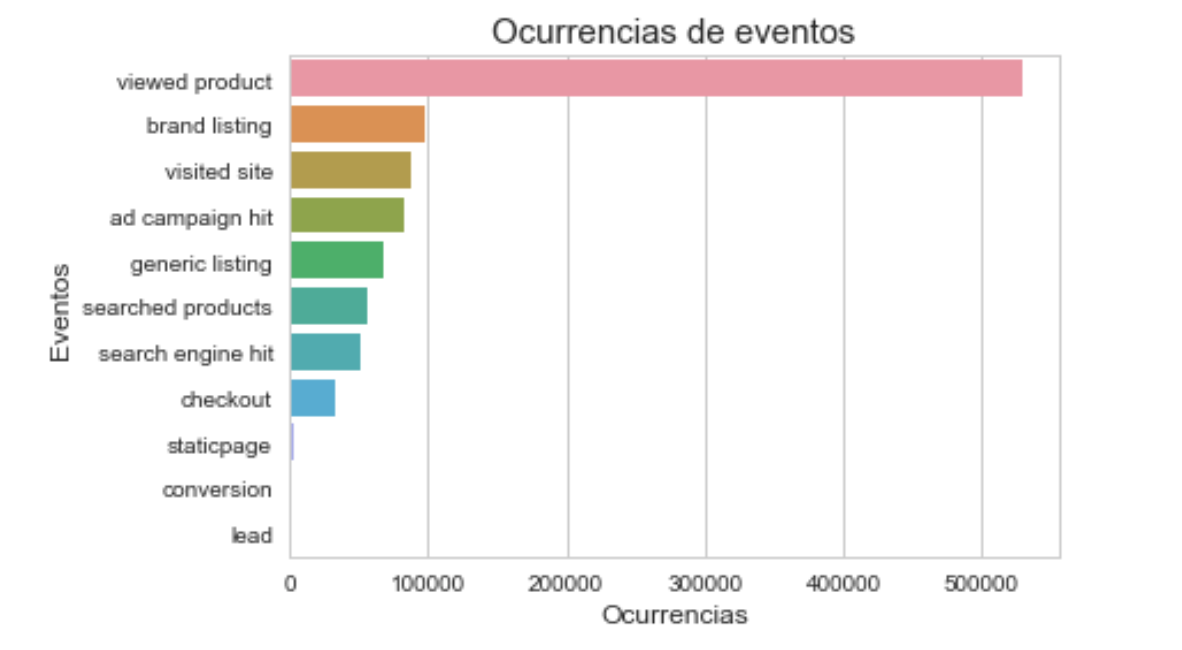
\includegraphics[width=10cm]{ocurrencia_eventos.jpg}\\
	\textbf{Figura 1:}  \textit{Cantidad de apariciones de cada evento. }
	\end{center}
	Nos dimos cuenta que no todos los campos del data participan en todos los eventos. Cada evento utiliza una determinada cantidad de columnas del data set. Por lo tanto, mediante un análisis de elementos nulos llegamos a las siguiente conclusiones:
	\begin{itemize}
		\item Todos los eventos tienen información temporal y sobre la persona que realizó dicho evento. 
		\item Para el evento \textbf{viewed product} sus campos obligatorios son: timestamp , sku , model, condition, storage, color.
		\item Para el evento \textbf{brand listing} su campo obligatorio es: skus. 
		\item Para el evento \textbf{visited site} sus campos obligatorios son: channel, new vs returning, city, region, country, device tipe , screen resolution, operating system version y browser version.
		\item Para el evento \textbf{ad campaing hit} sus campos obligatorios son: url  y campaing source.
		\item Para el evento \textbf{generic listing} su campo obligatorios es: skus.
		\item Para el evento  \textbf{serched product } sus campos obligatorios son: skus y search term.
		\item Para el evento \textbf{serched engine} su campo obligatorio es: search engine
		\item Para el evento \textbf{checked out}  sus campos obligatorios son: sku, color, storage, model y condition 
		\item Para el evento \textbf{static page}  sus campo obligatorio es: satatic page
		\item Para le evento \textbf{conversion} sus campos obligatorios son:  sku, model, color , condition y storage
		\item Para el evento \textbf{lead} su campo obligatorio es: model
	\end{itemize}	
	Como todos los eventos tienen información temporal. Decidimos análizar la cantidad de eventos que se realizan por hora del día y el resultado fue:
	\begin{center}
	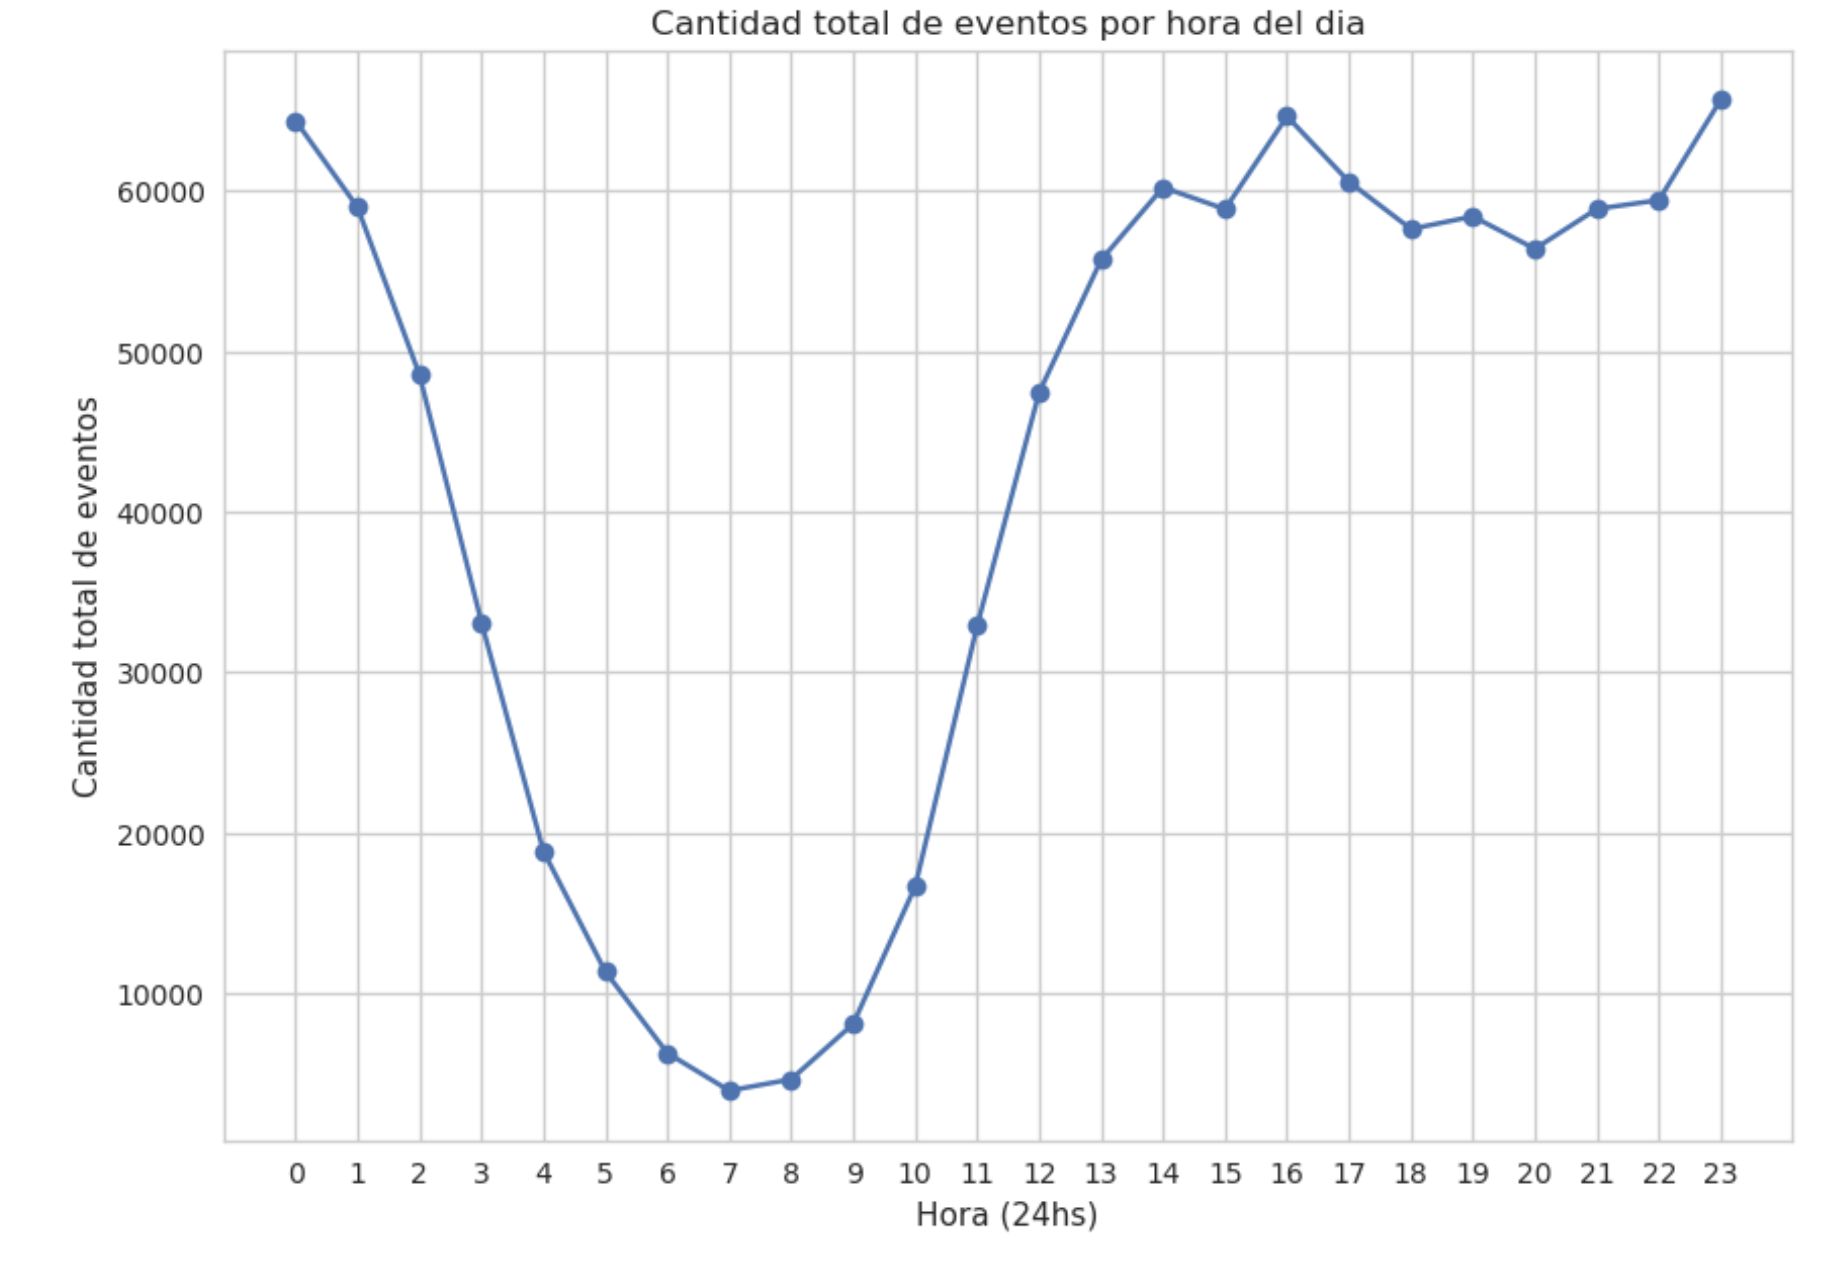
\includegraphics[width=10cm]{cantidadDeEventosPorHoraDelDia.jpg}\\
	\textbf{Figura 2:}  \textit{Distribución de los eventos a lo largo del día.}
	\end{center}
	Por lo tanto, la mayoría de los eventos se efectúan entre las 14 am y 2 am. \\
	\subsection{Viewed product}
	\subsubsection{Análisis individual de las características}
	La primera columna que decicimos analizar de éste evento es model. De ella obtuvimos los 15 celulares más vistos, ellos son:
	\begin{center}
	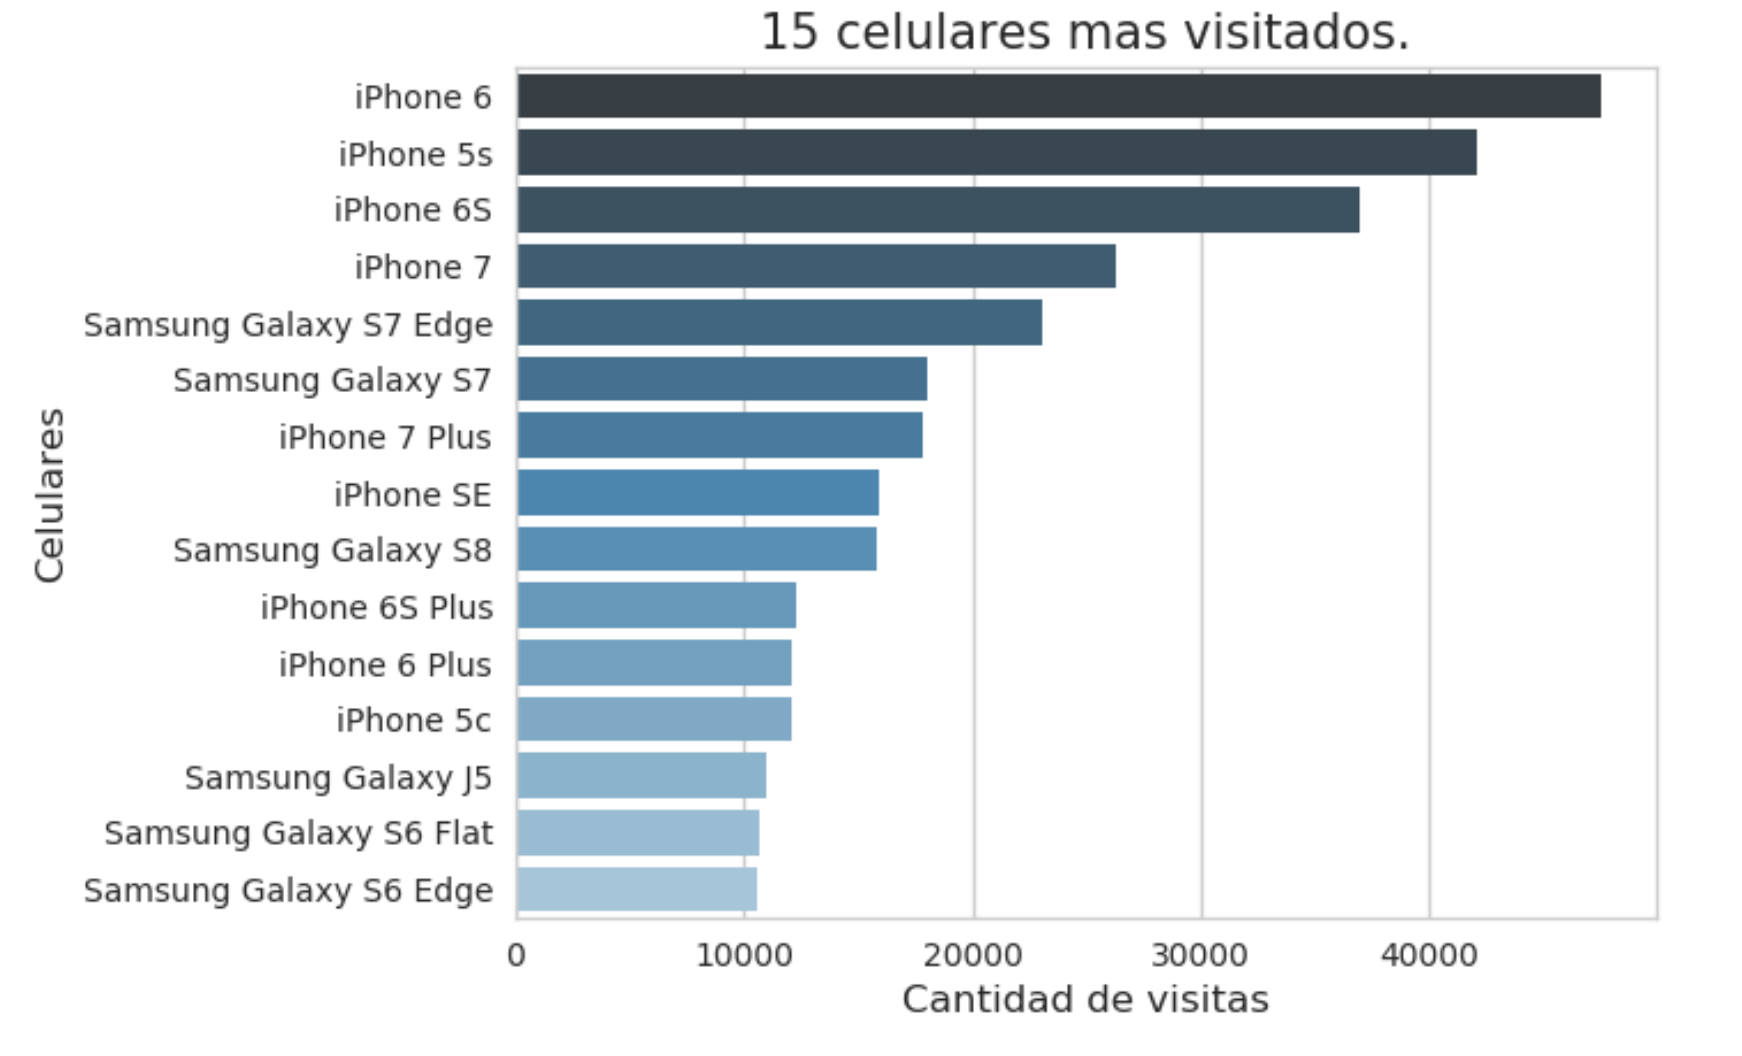
\includegraphics[width=10cm]{15celularesMasVisitados.jpg}\\
	\textbf{Figura 3:}  \textit{Cantidad de visitas por celular.}
	\end{center}
	 Sobre las características de esos modelos primero analizamos el color de los productos vistos y concluímos que: el 50\% de las visitas se concentraron en los siguientes colores:
	 Las visitas según el color de los celulares fue:
	\begin{itemize}
	\item el 23\% de las visitas es hacia productos negros.
	\item el 20\% de las visitas es hacia productos dorados.
	\item el 11\% de de las visitas es hacia productos gris espacial.
    \item el 10\% de de las visitas es hacia productos blancos.
     \item el 9\% de de las visitas es hacia productos plateados.
     \item el 6\% de de las visitas es hacia productos rosas.
     \item Despreciamos el resto de los colores ya que el porcentaje de visitas es poco significativo. 
	\end{itemize}	   
	Luego analizamos las visitas hacia el almacenamiento de los productos y concluímos que:
	\begin{itemize}
	\item El 33\% de las visitas es hacia productos con almacenamiento de 16 GB.
    \item El 32\% de las visitas es hacia productos con almacenamiento de 32 GB.
    \item El 17\% de las visitas es hacia productos con almacenamiento de 64 GB.
    \item El 6\% de las visitas es hacia productos con almacenamiento de 8 GB.
	\end{itemize}
	Por último analizamos las condiciones que más visita la gente y concluímos que:
	\begin{itemize}
    \item El 42\% de las visitas es hacia productos que son de calidad buena.
    \item El 27\% de las visitas es hacia productos que son de calidad excelente .
    \item El 27\% de las visitas es hacia productos que son de calidad muy buena.
        \item El 2\% de las visitas es hacia  productos que tienen identificador de huella digital. 
        	\item El 0,02\%  de las visitas es hacia  productos nuevos.    
	\end{itemize}
	Por otra parte, realizamos un análisis temporal sobre el evento y obtuvimos que:
	\subsubsection{Análisis temporal}
	\begin{center}
	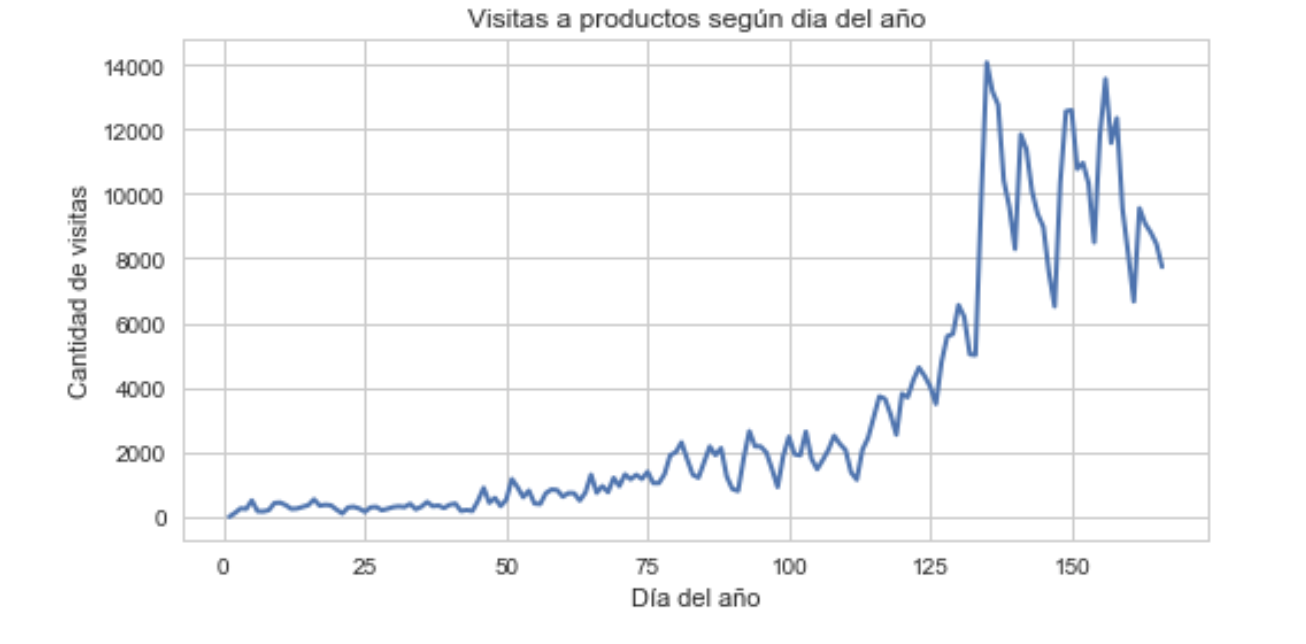
\includegraphics[width=10cm]{VisitasAProductosSegunDiaAnio.jpg}\\
	\textbf{Figura 4:}  \textit{Cantidad de visitas según día del año.  }
	\end{center}

	\begin{center}
	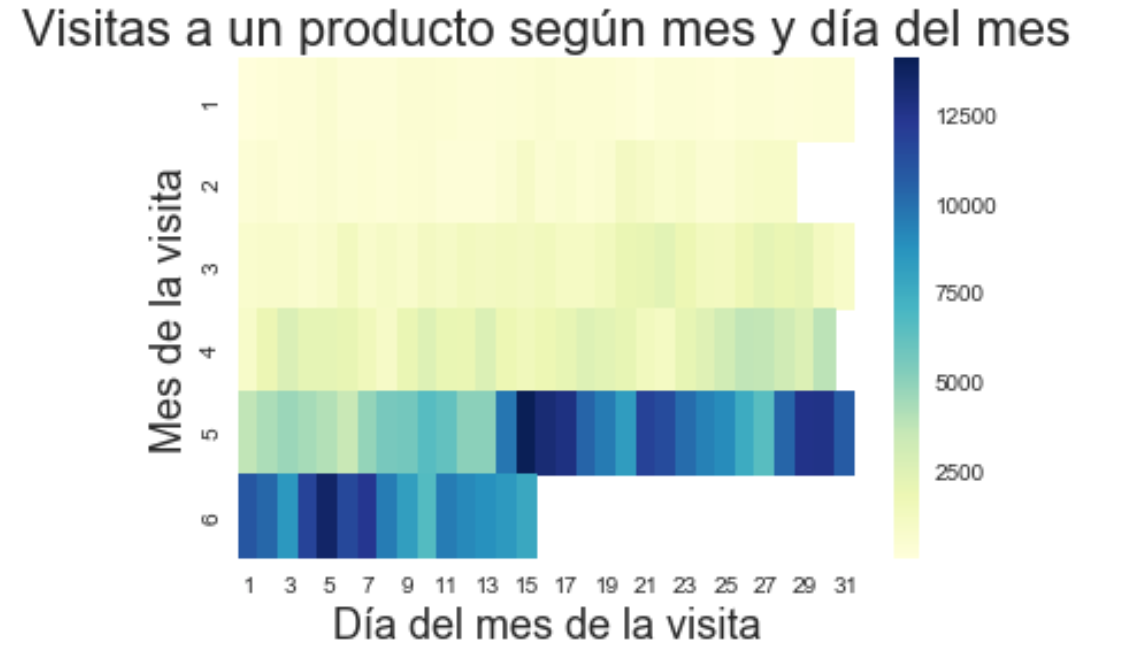
\includegraphics[width=10cm]{visitasSegunmesDiaMes.jpg}\\
	\textbf{Figura 5:}  \textit{Cantidad de visitas por cada día de cada mes. }\\
	Podemos notar que hay un fuerte incremento de actvidad a partir del 15 de mayo. 
	
	\end{center}
	\begin{center}
	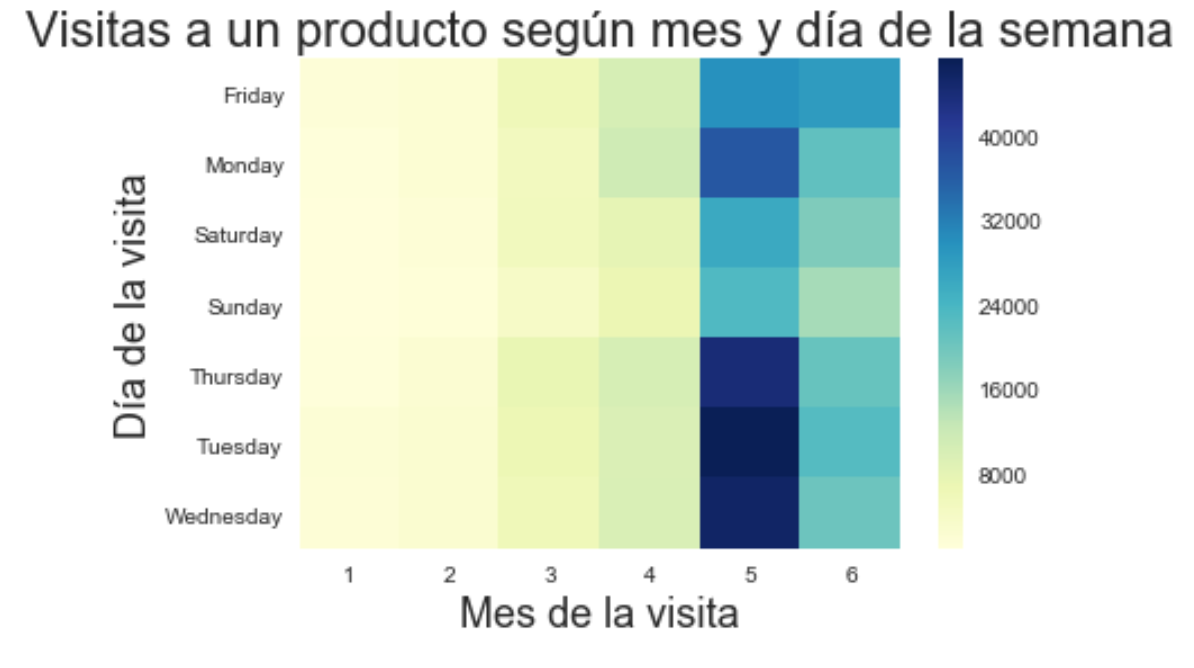
\includegraphics[width=10cm]{visitasSegunMesYDiaDeSemana.jpg}\\
	\textbf{Figura 6:}  \textit{Cantidad de visitas por cada día de semana de cada mes.   }
	\end{center}
	Nuevamente hay un fuerte incremento a partir del mes de mayo. Sin embargo, no parece haber una predominancia cuando hablamos de los días de la semana. Lo que podemos concluir es que los domingos hay menos actividad. 
	
	\textbf{Es importante destacar en el análisis temporal que el mes de  junio no está completo. Sólo tenemos datos de su primera quincena. }
	
	\subsubsection{Análisis cruzado}
	Por último relacionaremos todas las careacterísticas analizadas anteriormente entre sí. Primero entrelazaremos la inforamción entre los cinco modelos más vistos y su color. Obtuvimos lo siguiente:

	\begin{center}
	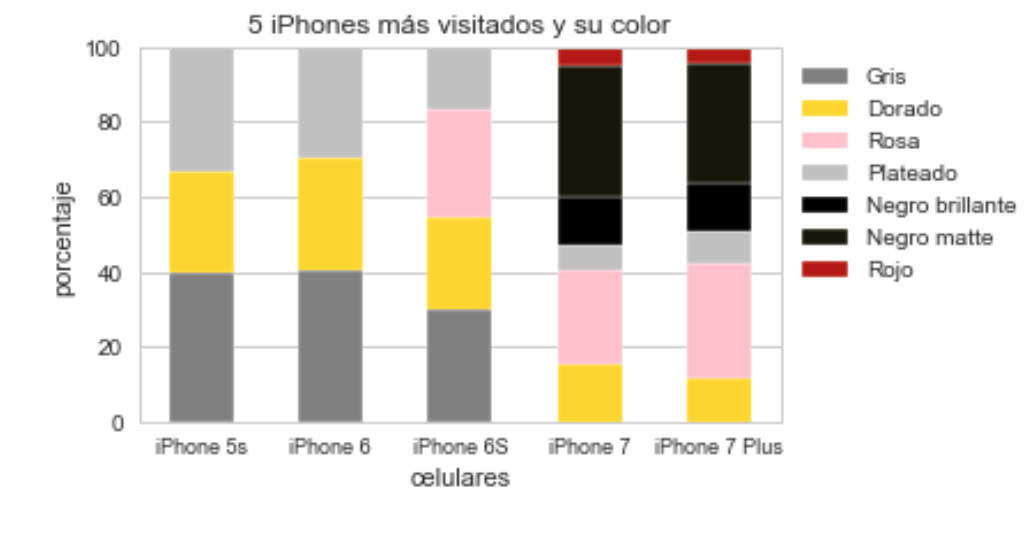
\includegraphics[width=10cm]{cincoModMasVisitadosColor.jpg}\\
	\textbf{Figura 7:}  \textit{Top 5 de celulares según su color. }
	\end{center}
	Por último, entrelazremos información entre los cinco modelos más visitos y su almacenamiento. Obtuvimos lo siguiente: 
	\begin{center}
	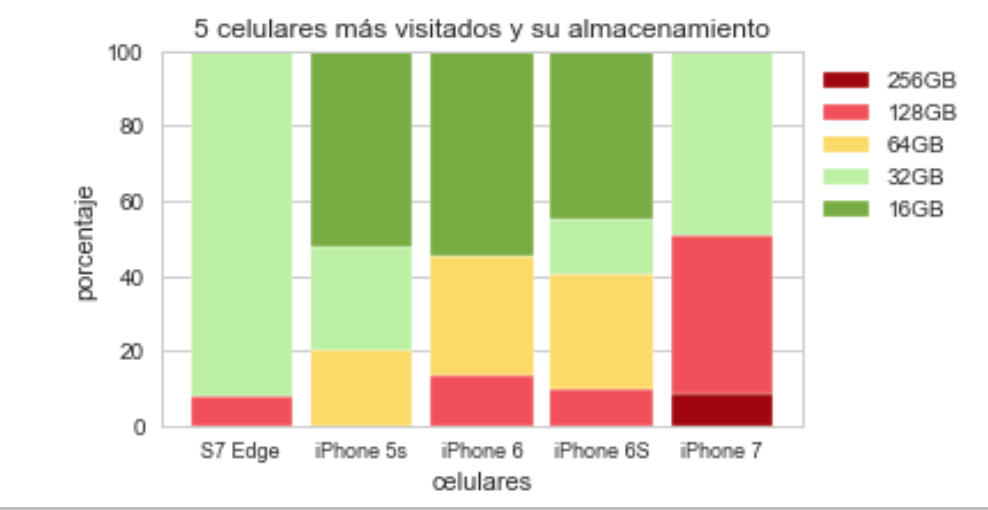
\includegraphics[width=10cm] {cincoModMasVisitadosAlmacenamiento.jpg}\\
	\textbf{Figura 8:}  \textit{Top 5 de celulares según su almacenamiento. }
	\end{center}


\textbf{[¿AGREGAR INFORMACIÓN SOBRE 5 TOP DE PRODUCTOS Y CONDICIÓN?
agregar explicación de porqué sólo se analizaron iphones en color.
]}
	
	
	\subsection{Ad campaign Hit}
	\subsubsection{Análisis individual de las caracterísiticas}
	Comenzamos analizando este evento fijandonos cuáles son las 10 campañas publicitarias más visitadas. Obtuvimos lo siguiente:
	\begin{center}
	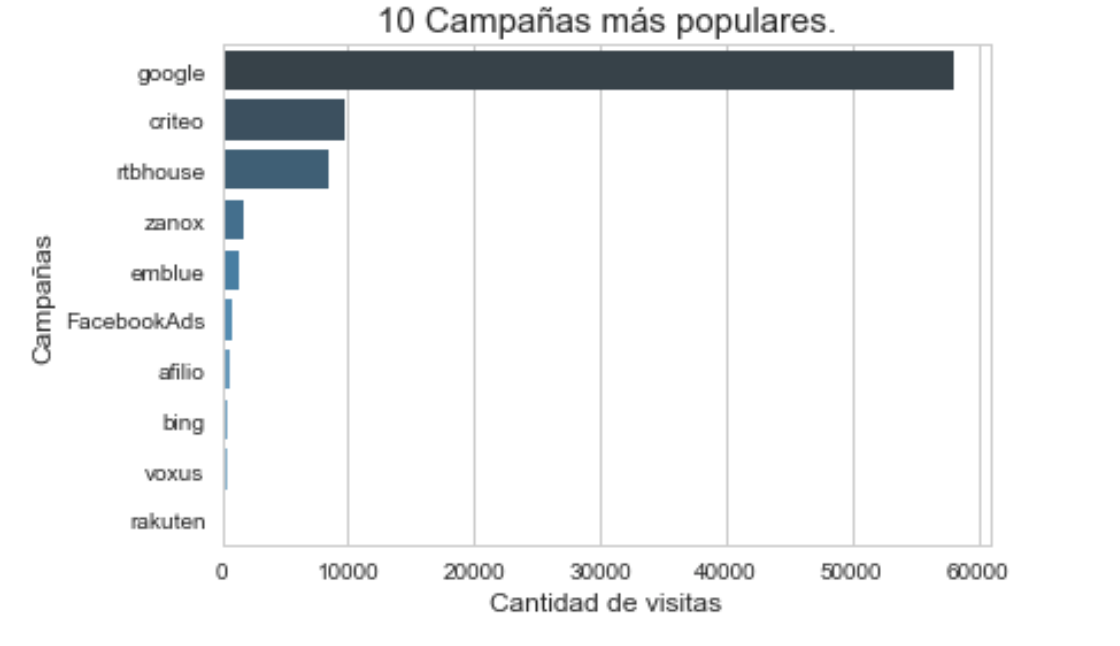
\includegraphics[width=10cm] {10campaniasmasPopulares.jpg}\\
	\textbf{Figura 9:}  \textit{En este gráfico se muestran las 10 campañas publicitarias más visitadas.  }
	\end{center}
	Ad campaign hit se divide en tres tipos de accesos: página principal, ventas y compras. Obtuvimos que: 
	\begin{itemize}
	\item El 65\% de los accesos es a compras.
	\item El 34\% de los accesos es a la página principal.
	\item El 0,26\% de los accesos es a ventas. 
	\end{itemize}
	El acceso según ventas puede clasificarse según la marca. Obtuvimos lo siguiente: 
	\begin{center}
	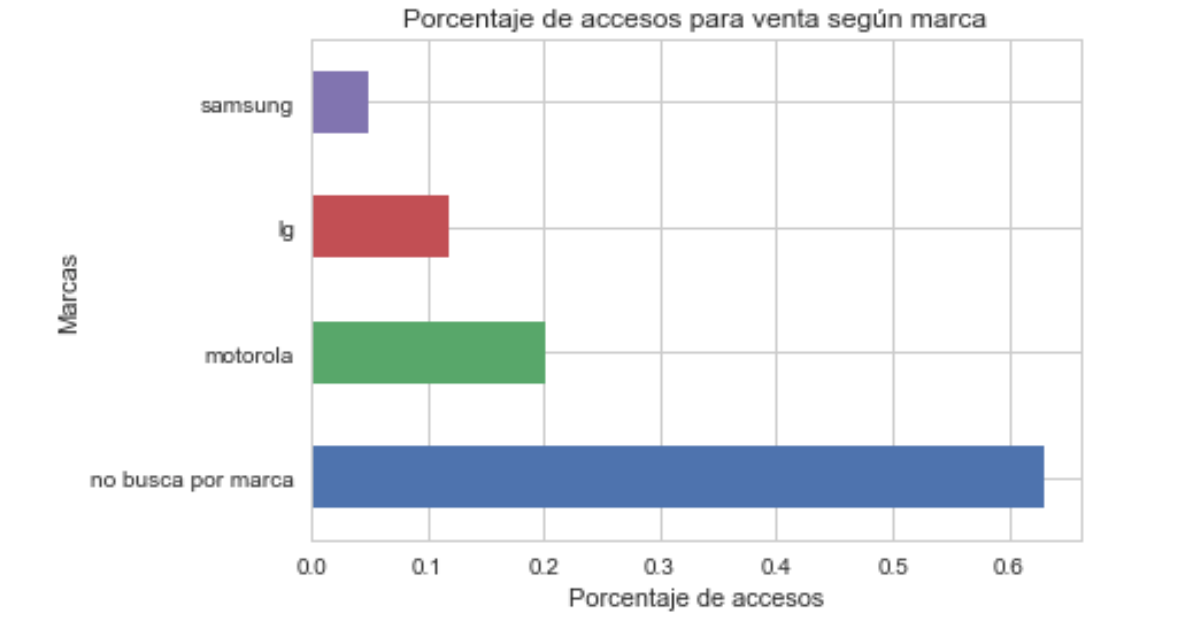
\includegraphics[width=10cm] {porcentajeDeAccesosParaVentaSegunMarca.jpg}\\
	\textbf{Figura 10:}  \textit{Porcentaje de accesos para venta según la marca.}
	\end{center}
	Este acceso tambien puede clasificarse según el modelo. Obtuvimos lo siguiente:
	\begin{center}
	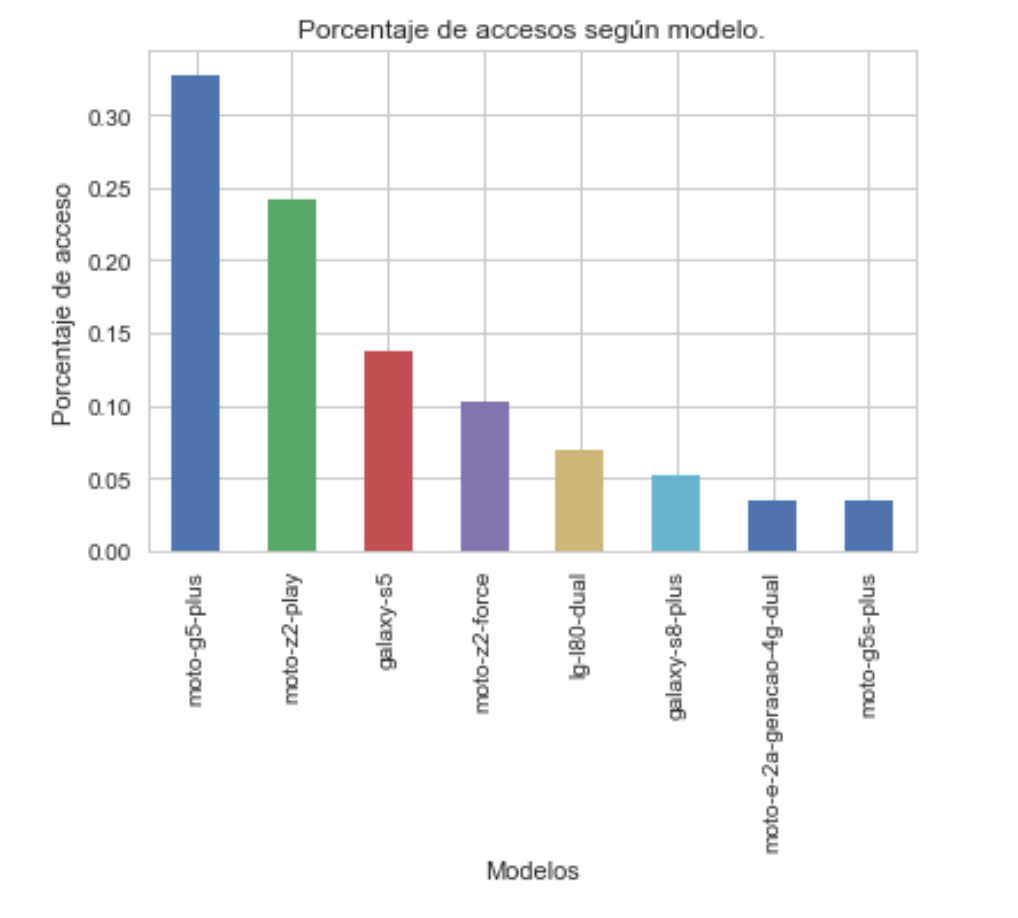
\includegraphics[width=10cm] {porcentajeDeAccesosSegunModelo.jpg}\\
	\textbf{Figura 11:}  \textit{Porcentaje de accesos para venta según el modelo.}
	\end{center}
	El acceso según compras puede clasificarse según la marca. Obtuvimos lo siguiente:
	\begin{center}
	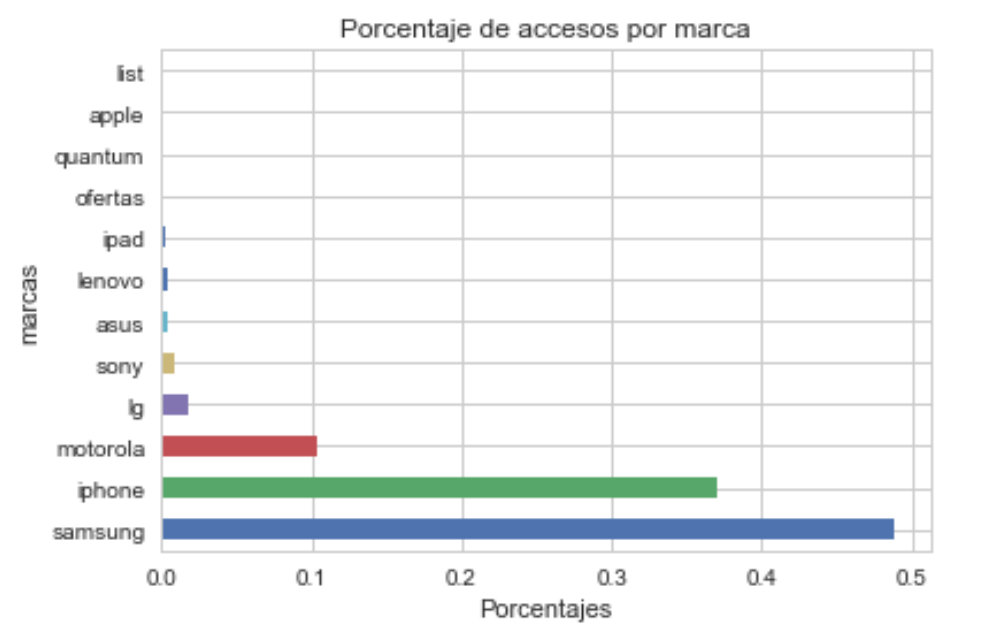
\includegraphics[width=10cm] {porcentajeDeAccesosPorMarcaSegunCompras.jpg}\\
	\textbf{Figura 12:}  \textit{Porcentaje de accesos para compra según la marca}
	\end{center}
	El acceso de compras por oferta es poco significativo. Por eso no lo excluyo del gráfico. 
	Hacer un análisis de las compras según modelo es muy complicado y no creemos que valga la pena. Esto se debe a que un mismo modelo puede tener urls distitntos. 
	\subsubsection{Análisis temporal}
	Luego, analizamos el top 5 de las campañas publicitarias más clickeadas, es decir, más visitadas según el mes. Obtuvimos lo siguiente: 
	\begin{center}
	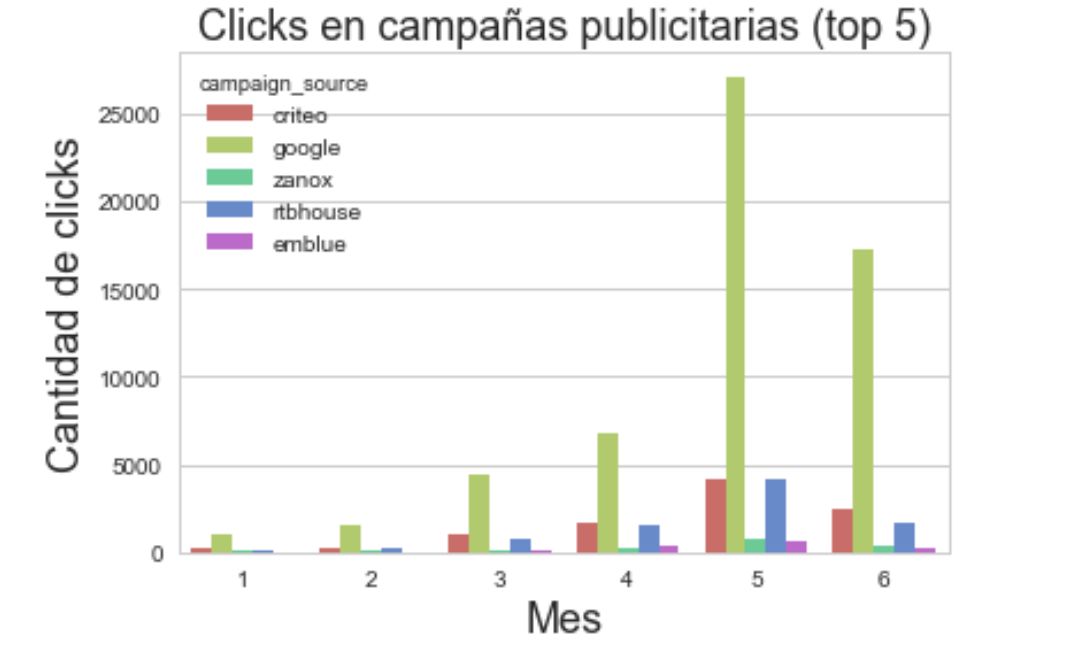
\includegraphics[width=10cm] {top5campaniasPublicitariasMasImportantesSegunMes.jpg}\\
	\textbf{Figura 13:}  \textit{Cantidad de clicks según campaña por mes.}
	\end{center}
	Analizamos así tambien el top5 de publicidades según la cantidad de clicks según el día del año. Obtuvimos lo siguiente:
	\begin{center}
	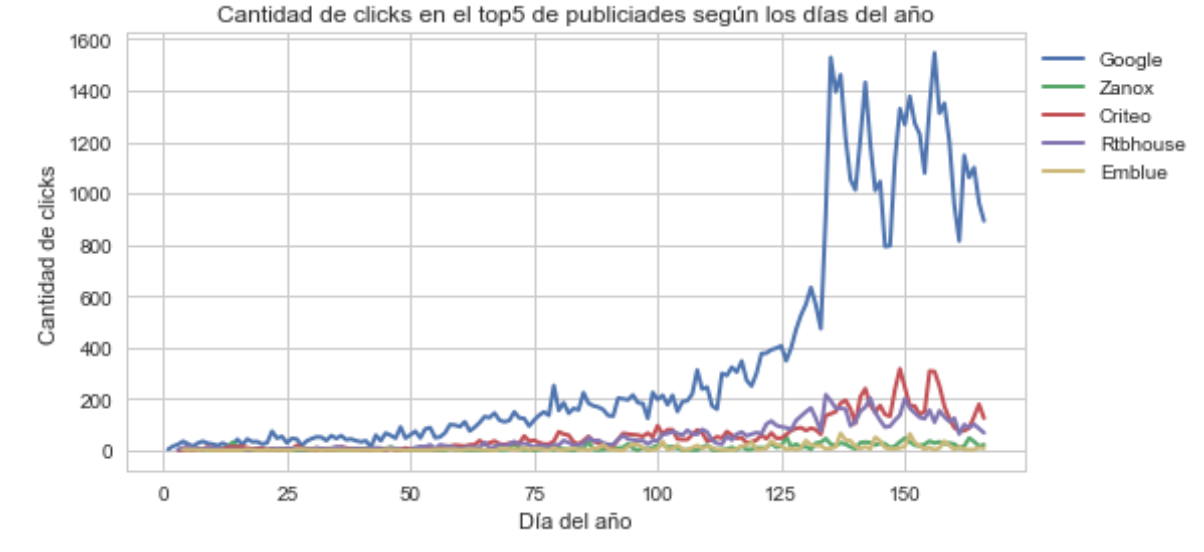
\includegraphics[width=10cm] {cantidadDeClicksSegunDiaDelAnio.jpg}\\
	\textbf{Figura 14:}  \textit{Cantidad de clicks según campaña por día del año.  }
	\end{center}
	\subsection{Checkout}
	\subsubsection{Análisis individual de las caracterísiticas}
	Empezamos analizando los 10 modelos que más llegaron al checkout. Ellos fueron:
	\begin{itemize}
	\item iPhone 6 con el 10\% de los checkouts.
	\item iPhone 5s con el 8\% de los checkouts.
	\item iPhone 6S  con el 7\% de los checkouts.
	\item Samsung Galaxy J5 con el 6\% de los checkouts.
	\item Samsung Galaxy S7 con el 4\% de los checkouts.
	\item iPhone 7 con el 4\% de los checkouts.
	\item Samsung Galaxy S8 con el 3\% de los checkouts.
	\item iPhone 7 Plus con el 3\% de los checkouts.
	\item Samsung Galaxy J7 Prime con el 3\% de los checkouts.
	\item Samsung Galaxy S6 Flatcon el 3\% de los checkouts.
	\end{itemize}
	Analizamos la cantidad de checkouts según el almacenamiento. Lo obtenido fue:
	\begin{itemize}
	\item El 37\% de los checkouts fue de dispositivos de 16GB
	\item El 29\% de los checkouts fue de dispositivos de 32GB
	\item	El 16\% de los checkouts fue de dispositivos de 64GB
	\item	El 11\% de los checkouts fue de dispositivos de 8GB
	\item	El 5\% de los checkouts fue de dispositivos de 128GB
	\item	El 1\% de los checkouts fue de dispositivos de 4GB
	\item	El 1\% de los checkouts fue de dispositivos de 256GB
	\item	El 0,1\% de los checkouts fue de dispositivos de 512MB
	\end{itemize}
	Analizamos la cantidad de checkouts según el color. Lo obtenido fue:
	\begin{center}
	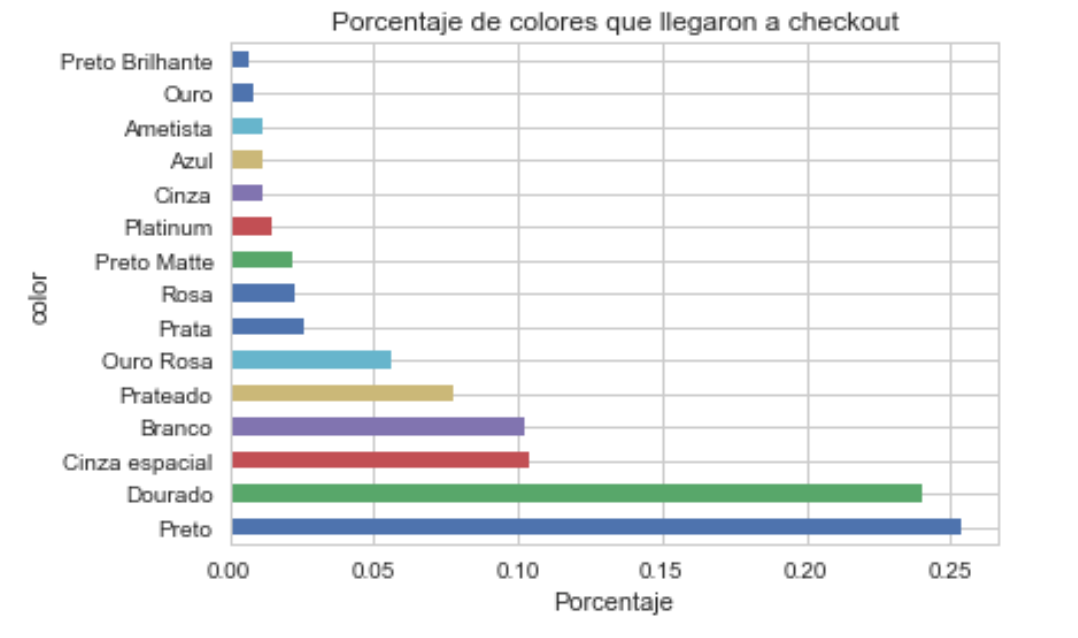
\includegraphics[width=10cm] {porcentajeDeColoresQueLlegaronACheck.jpg}\\
	\textbf{Figura 15:}  \textit{Porcentaje de colores que llegaron al checkout.}
	\end{center}
	Por último analizamos la calidad de los productos que llegaron al checkout. Lo obtenido fue:
	\begin{itemize}
	\item El 45 \% de los productos son de calidad buena. 
	\item El 27\% de los productos son de calidad excelente.
	\item El 24\% de los productos son de calidad muy buena. 
	\item El 3\% de los productos son de calidad buena con touch id. 
	\item No es representativo la cantidad de productos nuevos. 
	\end{itemize}
	\subsubsection{Análisis temporal}
	Analizamos la cantidad de checkouts según los días del año. Obtuvimos lo siguiente:
	\begin{center}
	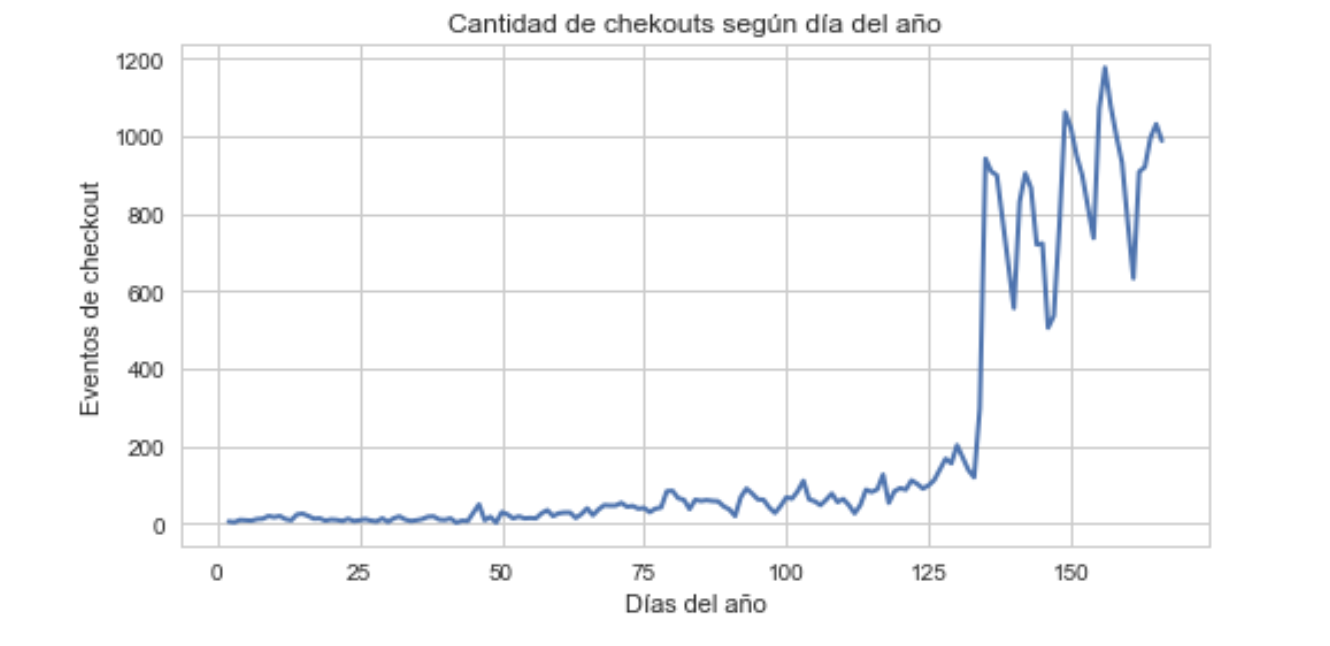
\includegraphics[width=10cm] {cantidadDeCheckoutsSegunDiaDelAnio.jpg}\\
	\textbf{Figura 15:}  \textit{Cantidad de checkouts según día del año.}
	\end{center}
	
	\subsubsection{Análisis cruzado}
	
	
	
	
	
	
	

	
	
	
\end{document}